\chapter{Overview of the Previous Work}

\section{The history of Self Organizing Map (SOM)}
Self-Organizing Map (SOM), also know as Kohonen map, is a topological preserving map that can map a higher dimensional space to a lower dimensional space. Along this process, information will be compressed; while, the key parameters in terms of "topological and metric relationships"\cite{Kohonen1998} will be retained. 
\\
There are two steps involved in forming a self-organizing map from a raw input data-set\cite{hebbian2007}, respectively to be 1) \textbf{competition} and 2) \textbf{cooperation}. When a set of data is feed into the system sequentially with random shuffle, for each input data point, \textbf{competition} will take place first and, based on a pre-defined cost function, one of the neurons on the output layer with the minimal cost will be selected as a winner; Following the competition, the  \textbf{cooperation} will then take place. Based on a neighborhood function, the winner together with it's neighbor neurons will proceed the learning; while, the neurons outside of the winner's neighbor zone will gain no learning. The purpose of the cooperation step is to increase the like-hood that if a similar input pattern present again, the same group of neurons will become the winner with a higher possibility. Iterate with this strategy on the input data-set over a suitable period, without supervising (providing error to the system), the output layer will simultaneously form a map that contains the similar topological structure as the input data. 

\section{Simon and his two methods}
In 2006, Simon and his Phd student published two very important papers for this task scheduling problem.

\begin{figure}[h]
  \centering
  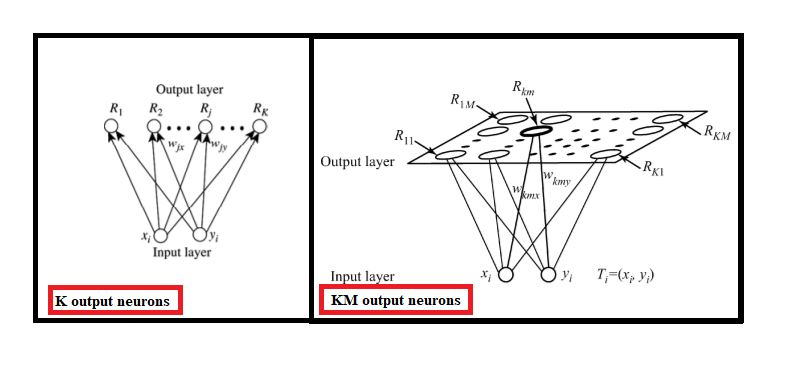
\includegraphics[width=15cm]{Pictures/SimonAmin2Methods.JPG}
  \caption{The illustration of two SOM configuration\cite{zhu2006neural,zhu2006k}.}
  \Description{The figure on the left has $K$ neurons on the output layer\cite{zhu2006k}; while, the figure on the right has $KM$ neurons on the output layer\cite{zhu2006neural}}
\end{figure}

\subsection{A simple SOM with $K$ output neurons}
\subsection{The impletation, SOM with $KM$ output neurons}